\documentclass[11pt,a4paper]{article}
%%%----------------------------------------------------------------------------%%%
%%%----------------------------------------------------------------------------%%%
%%% 
%%% ### Packages 
%%%
%%%----------------------------------------------------------------------------%%%
%%%----------------------------------------------------------------------------%%%
\usepackage{amsmath, amsthm, amssymb, nccbbb, bm, dsfont, pifont, fontawesome, graphicx, varioref, enumitem, mathtools, listings, xcolor, cite, fancyhdr, lastpage, lscape, subfig, graphicx, float, tabularx, algpseudocode, algorithm, multirow, setspace, hyperref, tabularx}

\RequirePackage[round,authoryear]{natbib}
\RequirePackage[colorlinks,citecolor=blue,urlcolor=blue]{hyperref}
\usepackage[cal=boondox]{mathalfa}
%\usepackage[numbers]{natbib}
\setlength{\topmargin}{-0.2in}
\setlength{\textheight}{9.2in}
\setlength{\oddsidemargin}{-.4in}
\setlength{\textwidth}{7in}
\hypersetup{colorlinks=true, linkcolor=blue, citecolor=red, urlcolor=blue}

% \onehalfspacing
\doublespacing

%%%----------------------------------------------------------------------------%%%
%%%----------------------------------------------------------------------------%%%
%%% 
%%% ### Code 
%%%
%%%----------------------------------------------------------------------------%%%
%%%----------------------------------------------------------------------------%%%
\usepackage{listings}
\lstset{escapeinside=| |}
\usepackage[usenames,dvipsnames]{color}  
\definecolor{mygray}{rgb}{0.99,0.99,0.99}
\definecolor{myblue}{rgb}{0.0, 0.23, 0.63}
\definecolor{myred}{rgb}{0.75, 0.0, 0.0}
\definecolor{mygreen}{rgb}{0.4, 0.69, 0.2}  
\lstnewenvironment{R}{\lstset{ 
  language=R,
  basicstyle=\footnotesize\ttfamily, 
  numbers=left,
  numberstyle=\tiny\color{black},
  stepnumber=1,
  numbersep=5pt,
  backgroundcolor=\color{mygray},
  showspaces=false, 
  showstringspaces=false,
  showtabs=false, 
  frame=single,  
  rulecolor=\color{black},
  tabsize=4,
  captionpos=b,
  breaklines=true,
  breakatwhitespace=false,
  keywordstyle=\ttfamily\bfseries\color{myblue},
  commentstyle=\ttfamily\bfseries\color{myred},
  stringstyle=\ttfamily\bfseries\color{mygreen}
} 
}{}

%New colors defined below
\definecolor{codegreen}{rgb}{0,0.6,0}
\definecolor{codegray}{rgb}{0.5,0.5,0.5}
\definecolor{codepurple}{rgb}{0.58,0,0.82}
\definecolor{backcolour}{rgb}{0.95,0.95,0.92}

%Code listing style named "mystyle"
\lstdefinestyle{mystyle}{
  backgroundcolor=\color{backcolour}, commentstyle=\color{codegreen},
  keywordstyle=\color{magenta},
  numberstyle=\tiny\color{codegray},
  stringstyle=\color{codepurple},
  basicstyle=\ttfamily\footnotesize,
  breakatwhitespace=false,         
  breaklines=true,                 
  captionpos=b,                    
  keepspaces=true,                 
  numbers=left,                    
  numbersep=5pt,                  
  showspaces=false,                
  showstringspaces=false,
  showtabs=false,                  
  tabsize=2
}

%"mystyle" code listing set
\lstset{style=mystyle}

%%%----------------------------------------------------------------------------%%%
%%%----------------------------------------------------------------------------%%%
%%% 
%%% ### Box
%%%
%%%----------------------------------------------------------------------------%%%
%%%----------------------------------------------------------------------------%%%
\usepackage{tcolorbox}
\tcbuselibrary{breakable}
\newtcolorbox{mybox}{colback=yellow!5!white, colframe=gray!60!black, breakable}
\newtcolorbox{mybox0}{colback=white, colframe=gray!60!black, breakable}
	

%%%----------------------------------------------------------------------------%%%
%%%----------------------------------------------------------------------------%%%
%%% 
%%% ### Theorem style structures 
%%%
%%%----------------------------------------------------------------------------%%%
%%%----------------------------------------------------------------------------%%%
\numberwithin{equation}{section}
\theoremstyle{plain}
\newtheorem{theorem}{Theorem}[section]
\newtheorem{lemma}[theorem]{Lemma}
\newtheorem{corollary}[theorem]{Corollary}
\newtheorem{proposition}[theorem]{Proposition}
\newtheorem{condition}{Condition}[section]
\newtheorem{definition}{Definition}[section]
\theoremstyle{definition}
\newtheorem{example}{Example}[section]
\newtheorem{exercise}{Exercise}[section]
\newtheorem{remark}{Remark}[section]
\newtheorem{remark0}{Remark}
\newtheorem{question}{Question}


%%%----------------------------------------------------------------------------%%%
%%%----------------------------------------------------------------------------%%%
%%% 
%%% ### Operators 
%%%
%%%----------------------------------------------------------------------------%%%
%%%----------------------------------------------------------------------------%%%
\newcommand{\pr}{\mathsf{P}} 
\newcommand{\E}{\mathsf{E}} 
\newcommand{\median}{\mathop{\mathsf{median}}}
\newcommand{\Cov}{{\mathsf{Cov}}} 
\newcommand{\Corr}{{\mathsf{Corr}}} 
\newcommand{\Var}{{\mathsf{Var}}}
\newcommand{\SD}{{\mathsf{SD}}}
\newcommand{\CV}{{\mathsf{CV}}}
\newcommand{\Bias}{{\mathsf{Bias}}}
\newcommand{\AMSE}{\operatorname{\mathsf{AMSE}}}
\newcommand{\MSE}{\operatorname{\mathsf{MSE}}}
\newcommand{\ARE}{\mathsf{ARE}}
\newcommand{\AV}{\mathsf{AV}}
\newcommand{\CRLB}{{\mathsf{CRLB}}}

\newcommand{\pCorr}{\text{P}}
\newcommand{\sCorr}{\text{S}}
\newcommand{\kCorr}{\text{K}}
\newcommand{\bdCorr}{\text{BD}}
\newcommand{\cCorr}{\text{C}}


\newcommand{\inD}{    \overset{ \textnormal{d}   }{\rightarrow} }
\newcommand{\inAS}{   \overset{ \textnormal{a.s.}   }{\rightarrow} }
\newcommand{\inP}{    \overset{ \textnormal{pr}    }{\rightarrow} }
\newcommand{\inLp}{   \overset{ \mathcal{L}^p }{\rightarrow} }
\newcommand{\inMSE}{  \overset{ \textnormal{qm} }{\rightarrow} }
\newcommand{\inQM}{   \overset{ \textnormal{qm} }{\rightarrow} }
\newcommand{\indep}{\protect\mathpalette{\protect\independenT}{\perp}}
\def\independenT#1#2{\mathrel{\rlap{$#1#2$}\mkern4mu{#1#2}}}
\newcommand{\iid}{\textsc{iid}} 
\newcommand{\simIID}{   \overset{ \iid   }{\sim} }
\newcommand{\simIND}{   \overset{ {\indep}   }{\sim} }


\newcommand{\Bern}{\textnormal{Bern}} 
\newcommand{\Unif}{\textnormal{Unif}} 
\newcommand{\Normal}{\textnormal{N}} 
\newcommand{\logNormal}{\textnormal{LN}} 
\newcommand{\Bin}{\textnormal{Bin}} 
\newcommand{\NB}{\textnormal{NB}} 
\newcommand{\HG}{\textnormal{HG}} 
\newcommand{\Geom}{\textnormal{Geom}} 
\newcommand{\Beta }{\textnormal{Beta}} 
\newcommand{\BetaBin}{\textnormal{Beta-Bin}}
\newcommand{\Ga}{\textnormal{Ga}} 
\newcommand{\Exp}{\textnormal{Exp}} 
\newcommand{\Expo}{\textnormal{Expo}} 
\newcommand{\Po}{\textnormal{Po}} 
\newcommand{\Multi}{\textnormal{Multi}} 
\newcommand{\student}{\textnormal{t}} 
\newcommand{\Cauchy}{\textnormal{Cauchy}} 
\newcommand{\Pareto}{\textnormal{Pareto}} 
\newcommand{\Laplace}{\textnormal{Laplace}} 
\newcommand{\Logistic}{\textnormal{Logistic}} 
\newcommand{\Dir}{\textnormal{Dir}} 
\newcommand{\DP}{\textnormal{DP}} 
\newcommand{\Inv}{\textnormal{Inv-}} 
\newcommand{\F}{\textnormal{F}} 
\newcommand{\sign}{\textnormal{sign}}
\newcommand{\rank}{\textnormal{rank}}


\newcommand{\RV}{\textsc{rv}}
\newcommand{\cdf}{\textsc{cdf}} 
\newcommand{\cgf}{\textsc{cgf}} 
\newcommand{\pdf}{\textsc{pdf}} 
\newcommand{\pmf}{\textsc{pmf}} 
\newcommand{\chf}{\textsc{chf}} 
\newcommand{\mgf}{\textsc{mgf}}
\newcommand{\EF}{\textsc{EF}}
\newcommand{\NEF}{\textsc{NEF}}
\newcommand{\MLE}{\textsc{mle}}
\newcommand{\MAP}{\textsc{MAP}}
\newcommand{\Med}{\textsc{Med}}
\newcommand{\MME}{\textsc{mme}}
\newcommand{\QME}{\textsc{qme}}
\newcommand{\UMVUE}{\textsc{umvue}}
\newcommand{\MPT}{\textsc{MPT}}
\newcommand{\UMPT}{\textsc{UMPT}}
\newcommand{\LRT}{\textsc{LRT}}


\newcommand{\diag}{\mathop{\mathrm{diag}}}
\newcommand{\tr}{\mathop{\mathrm{tr}}}
\newcommand{\T}{\mathop{\mathrm{T}}}
\DeclareMathOperator*{\argmin}{arg\,min}
\DeclareMathOperator*{\argmax}{arg\,max}
\DeclareMathOperator{\sgn}{sgn}
\DeclareMathOperator{\logit}{logit}
\DeclareMathOperator{\expit}{expit}
\newcommand{\dd}{\textnormal{d}}


\newcommand{\lva}{{\color{myred}\ding{73}\ding{73}\ding{73}}}
\newcommand{\lvb}{{\color{myred}\ding{72}\ding{73}\ding{73}}}
\newcommand{\lvc}{{\color{myred}\ding{72}\ding{72}\ding{73}}}
\newcommand{\lvd}{{\color{myred}\ding{72}\ding{72}\ding{72}}}
\newcommand{\optional}{\noindent{\color{myblue}\faScissors}}
\newcommand{\Solution}{\noindent{\color{myblue}{{\textsc{Solution}}:~$\Big.$}}}
\newcommand{\take}{\noindent{\color{myblue}\faPaperPlaneO~\underline{\bf Takeaway}:~$\Big.$}}

% widecheck 
\DeclareFontFamily{U}{mathx}{\hyphenchar\font45}
\DeclareFontShape{U}{mathx}{m}{n}{
      <5> <6> <7> <8> <9> <10>
      <10.95> <12> <14.4> <17.28> <20.74> <24.88>
      mathx10
      }{}
\DeclareSymbolFont{mathx}{U}{mathx}{m}{n}
\DeclareFontSubstitution{U}{mathx}{m}{n}
\DeclareMathAccent{\widecheck}{0}{mathx}{"71}
\DeclareMathAccent{\wideparen}{0}{mathx}{"75}

\def\cs#1{\texttt{\char`\\#1}}

% Customize header and footer
\pagestyle{fancy}
\fancyhf{}
\fancyhead[L]{2022-23 Semester 2}
\fancyhead[R]{NSCI 4051 – Workshop on Data Sciences}
\fancyfoot[R]{Page \thepage\ of \pageref*{LastPage}}
% \fancyfoot[L]{\nouppercase{\leftmark}}
\renewcommand{\headrulewidth}{0.4pt} % default is 0pt
\renewcommand{\footrulewidth}{0.4pt} % default is 0pt

\usepackage[bottom]{footmisc}

\newcounter{magicrownumbers}
\newcommand\rownumber{\stepcounter{magicrownumbers}\arabic{magicrownumbers}}

\usepackage[table]{xcolor}
%------------------------------------------------------------------------------

\begin{document}
    
    % Page 0 for names and table of contents
    \thispagestyle{empty}
    \pagenumbering{gobble} 
    \title{\textsc{NSCI 4051} -- Workshop on Data Sciences}
    \author{
        LAW Yiu Leung Eric (SID: \texttt{1155149315})
    }
    \date{\today}
    \maketitle

    \begin{center}
        {\Large \textbf{Topic: Predict Student Performance from Time Series Data}} \\
        Instructor: Dr. Edmond Chan
    \end{center}
    
    \pagestyle{plain} 
    % \pagenumbering{roman}
    
    \tableofcontents
    \listoffigures
    \listoftables
    
    \newpage

    % \onehalfspacing
    % Section 1
    \pagenumbering{arabic}
    \pagestyle{fancy}
    \setcounter{page}{1}
    
    % Emotion Detection
    \section{Introduction}
    Game-based learning is a method of education that has seen growing popularity in recent years. It involves using gaming elements and mechanics to teach academic concepts and skills, making learning a more interactive and entertaining experience for students. This approach to education has been shown to be effective in engaging students and improving their academic outcomes. \\
    \\
    The lack of knowledge tracing in game-based learning platforms is a missed opportunity to provide individualized support to students, which can ultimately improve their academic outcomes. Therefore, there is a need for increased focus on incorporating knowledge tracing techniques in educational games to support students' learning and development. \\
    \\
    The project is trying to make advancement of knowledge-tracing methods for game-based learning. This will benefit the developers of educational games by providing them with valuable insights on how to create more effective learning experiences for their students. Ultimately, this work aims to enhance the quality of education through the use of game-based learning and promote better academic outcomes for students.

    \section{Dataset}
    \href{https://www.kaggle.com/competitions/predict-student-performance-from-game-play/overview}{Predict Student Performance from Game Play} from Kaggle uses the Kaggle's time series API. Test data will be delivered in groupings that do not allow access to future data. The objective is to use time series data generated by an online educational game, \href{https://pbswisconsineducation.org/jowilder/about/}{Jo Wilder and the Capitol Case}\footnote{A game based learning designed by PBS Wisconsin Education targeting child to learn English, history and arts.} \cite{jo_wilder}, to determine whether players will answer questions correctly. There are three question checkpoints (level 4, level 12, and level 22), each with a number of questions. At each checkpoint, you will have access to all previous test data for that section. \cite{game_date} There are 18 questions for each session, in \texttt{train\_labels.csv}, it told whether the user for a particular session answered each question correctly. \\
    \\
    \texttt{train.csv} contains 13,174,211 records with 20 features, the list of all features are included in appendix \hyperref[appendix:training]{Training Dataset Features}. 
    \\
    \begin{table}[H]
        \centering
        \begin{tabular}{l | l | l l}
        Filename               & Description                                                       & Rows       & Columns \\ \hline
        train.csv              & training dataset                                                  & 13,174,211 & 20      \\
        train\_labels.csv      & traning labels                                                    & 212,022    & 2       \\
        test.csv               & testing dataset                                                   & 3,728      & 21      \\
        sample\_submission.csv & sample of submission for prediction & 54 & 3       
        \end{tabular}
        \caption{Datasets}
        \label{tab:dataset}
    \end{table}
    \noindent
    Noted that \texttt{test.csv} and \texttt{sample\_submission.csv} are only for submission in Kaggle competition\footnote{Public competition that allows participants submit their prediction model.}, for the sake of simplicity of this project, those 2 datasets will be ignored in model development.

    \section{Exploratory Data Analysis}
    For complete and detailed exploratory data analysis, please refer to jupyter notebook \texttt{EDA.ipynb}, only important findings are included in this written report.

    \subsection{Missing Value}
    For \textit{page}, \textit{hover\_duration}, \textit{text} and \textit{text\_fqid}, they have high missing ratio over 60\%. We may consider to drop these features later, but still we have to evaluate the relevance of them. \\
    For \textit{fullscreen}, \textit{hq} and \textit{music}, they are completely missing and contain no information, therefore, they have to be dropped.
    \begin{figure}[H]
        \centering
        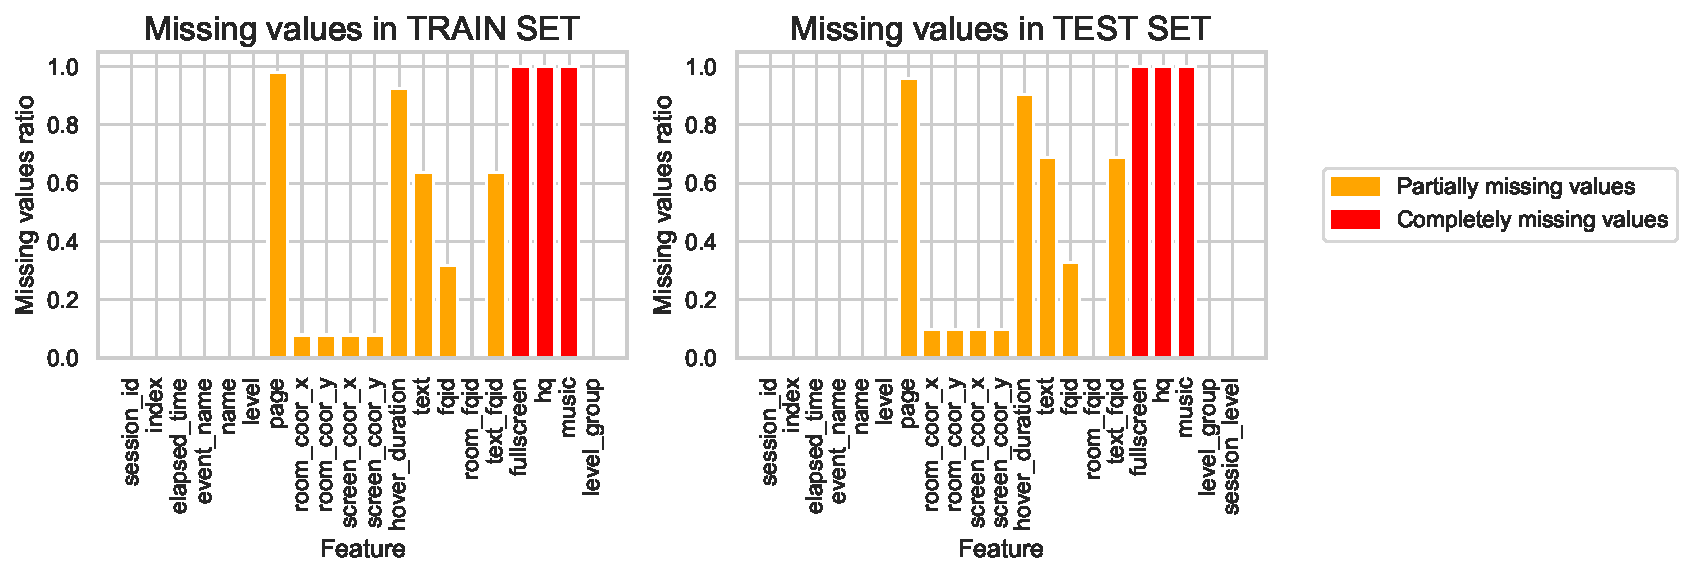
\includegraphics[width = 0.9\textwidth]{EDA_plot/missing_value.pdf}
        \caption{Missing Value}
        \label{fig:missing_value}
    \end{figure}

    \subsection{Session and Index}
    There are 11,179 unique sessions in training dataset, each session have different number of events in range of [634, 19032], both the mean and median are at around 1,100, where the distribution appears to be normal with little positive skew. The 90th percentile is around 1,500, however, some session contain over 10,000 events, we may consider it as outlier.
    \begin{figure}[H]
        \centering
        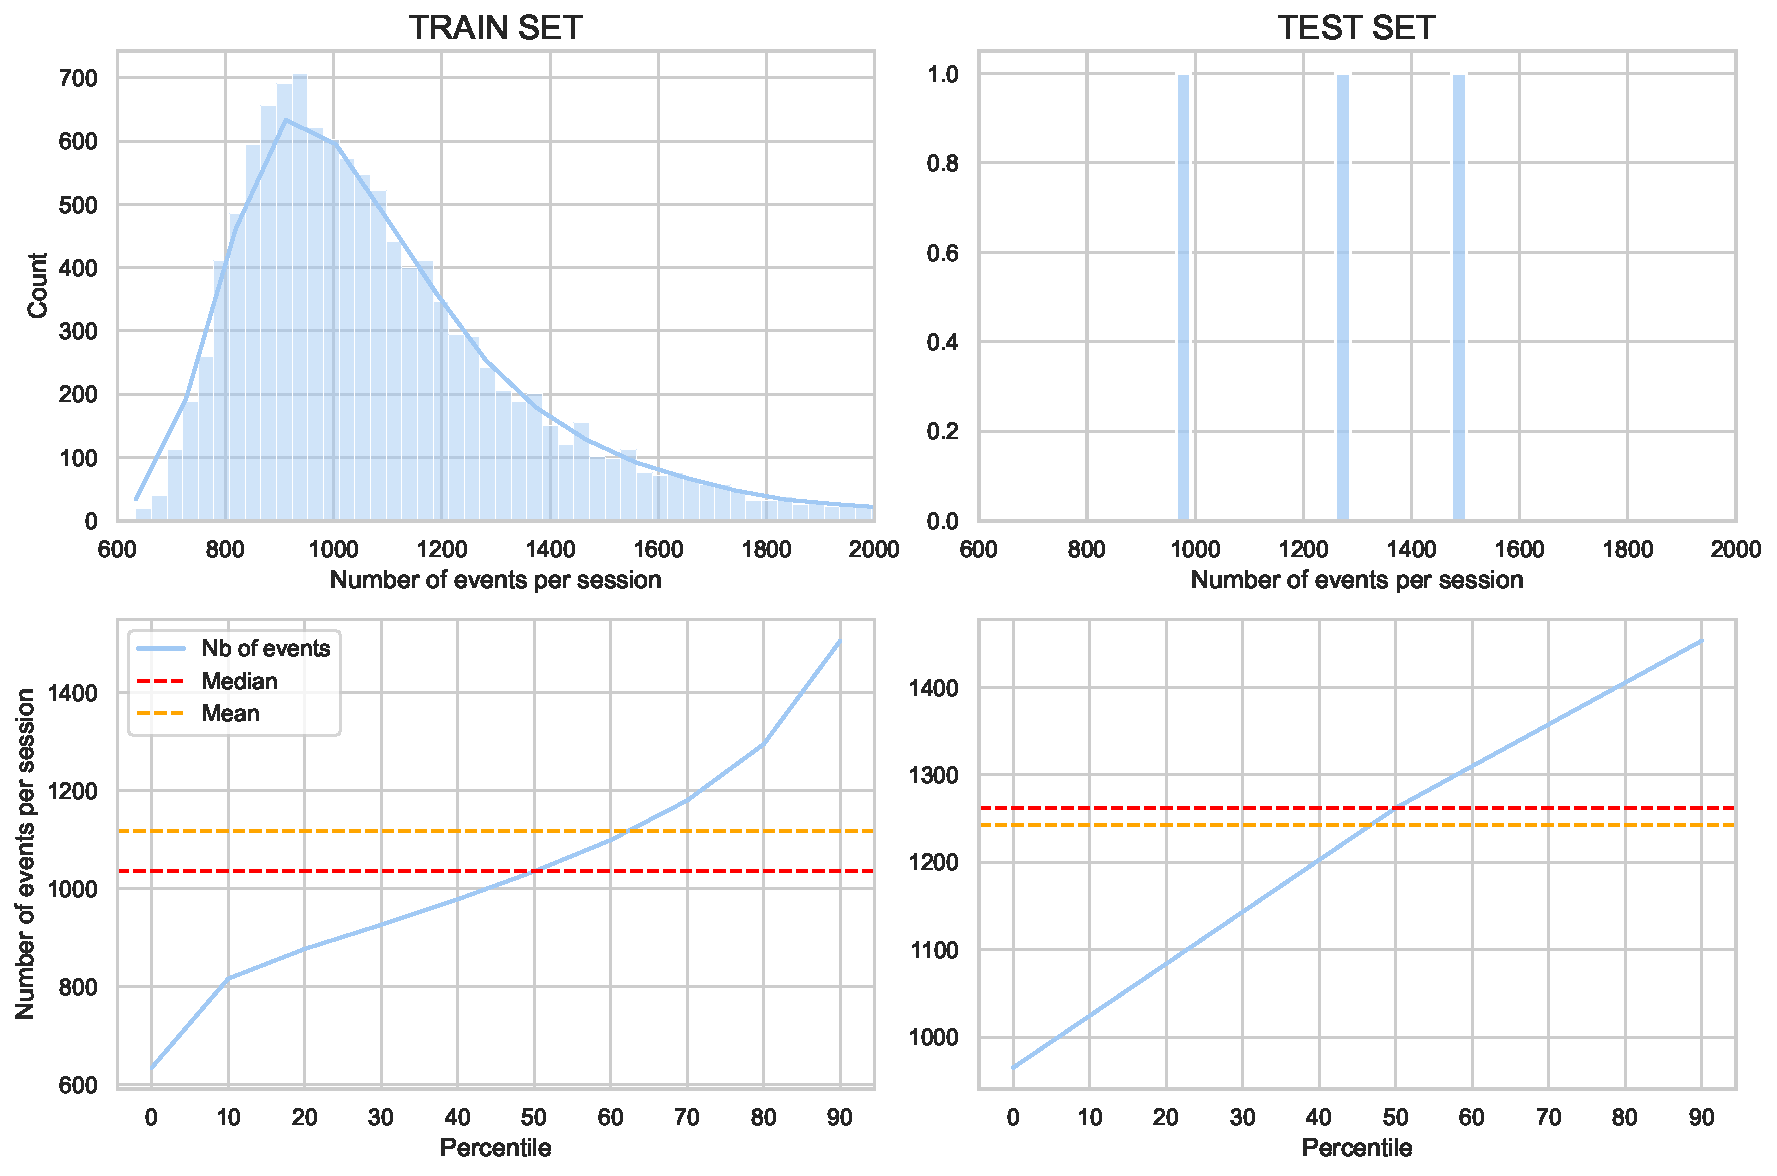
\includegraphics[width = 0.9\textwidth]{EDA_plot/no_events.pdf}
        \caption{Session and Index}
        \label{fig:no_events}
    \end{figure}

    \subsection{Elapsed Time}
    We may assume that elapsed time is positively correlated with the event index. As more time is spent, it is expected that a higher number of events will occur. \\
    The figure show as expected, the elapsed time increases as the event index increases, which have strong correlation until the event index 1600 and no more correlations after 2800. This phenomenon can be explained by number of samples for larger event indexes are dropping significantly, those are likely to be outliers. Figure \ref{fig:elapsed_time_outlier} shows 16 samples of outliers, most of the sessions have gaps between the increase of elapsed time, indicating pauses or inactivity. In the case of outlier sessions, the gap is huge due to extended periods of inactivity.
    \begin{figure}[H]
        \centering
        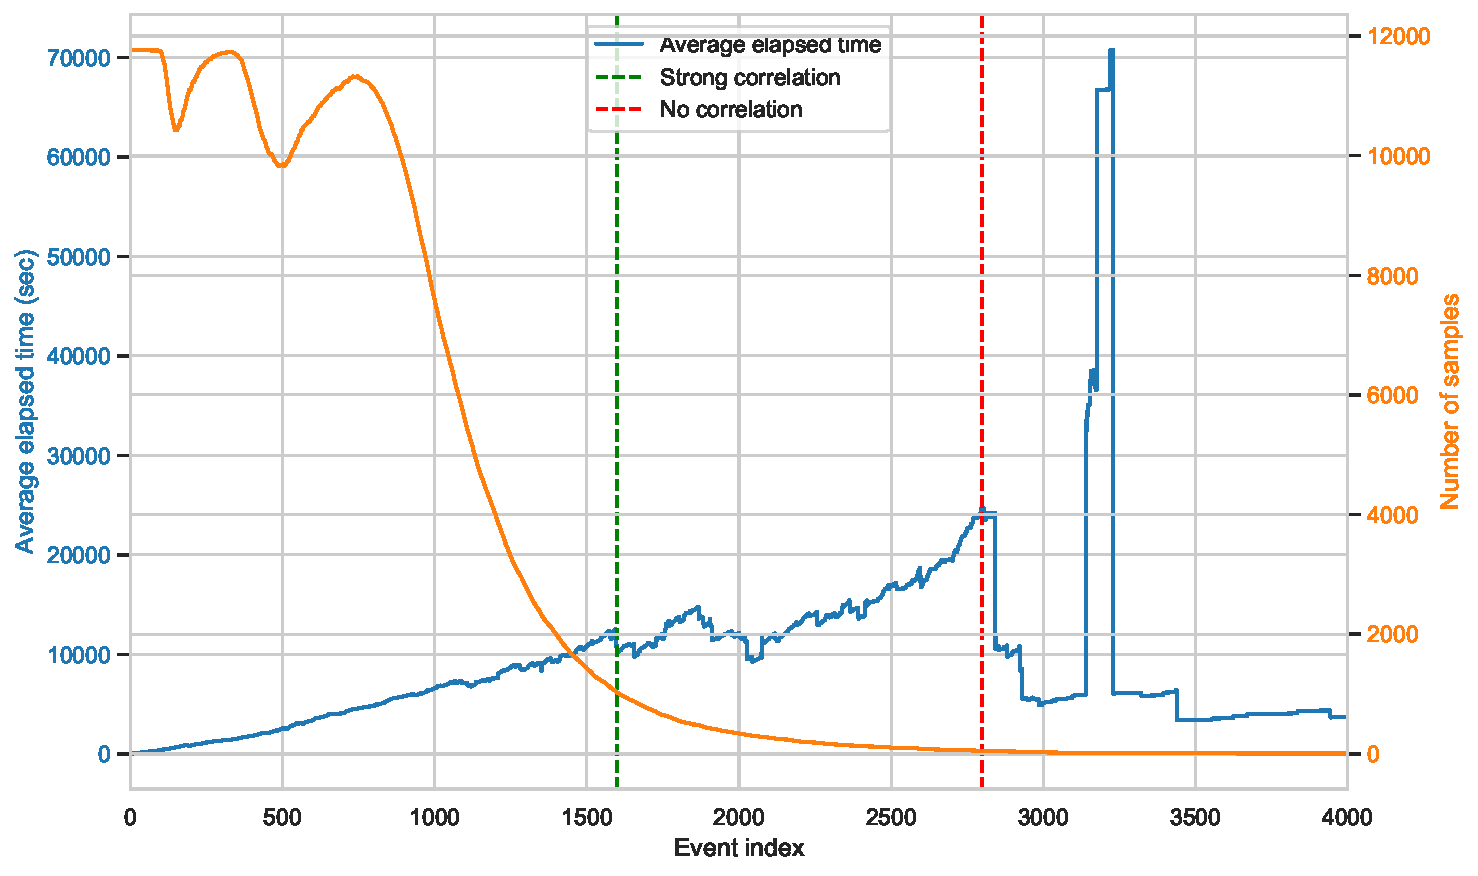
\includegraphics[width = 0.9\textwidth]{EDA_plot/elapsed_time.pdf}
        \caption{Elapsed Time}
        \label{fig:elapsed_time}
    \end{figure}
    \begin{figure}[H]
        \centering
        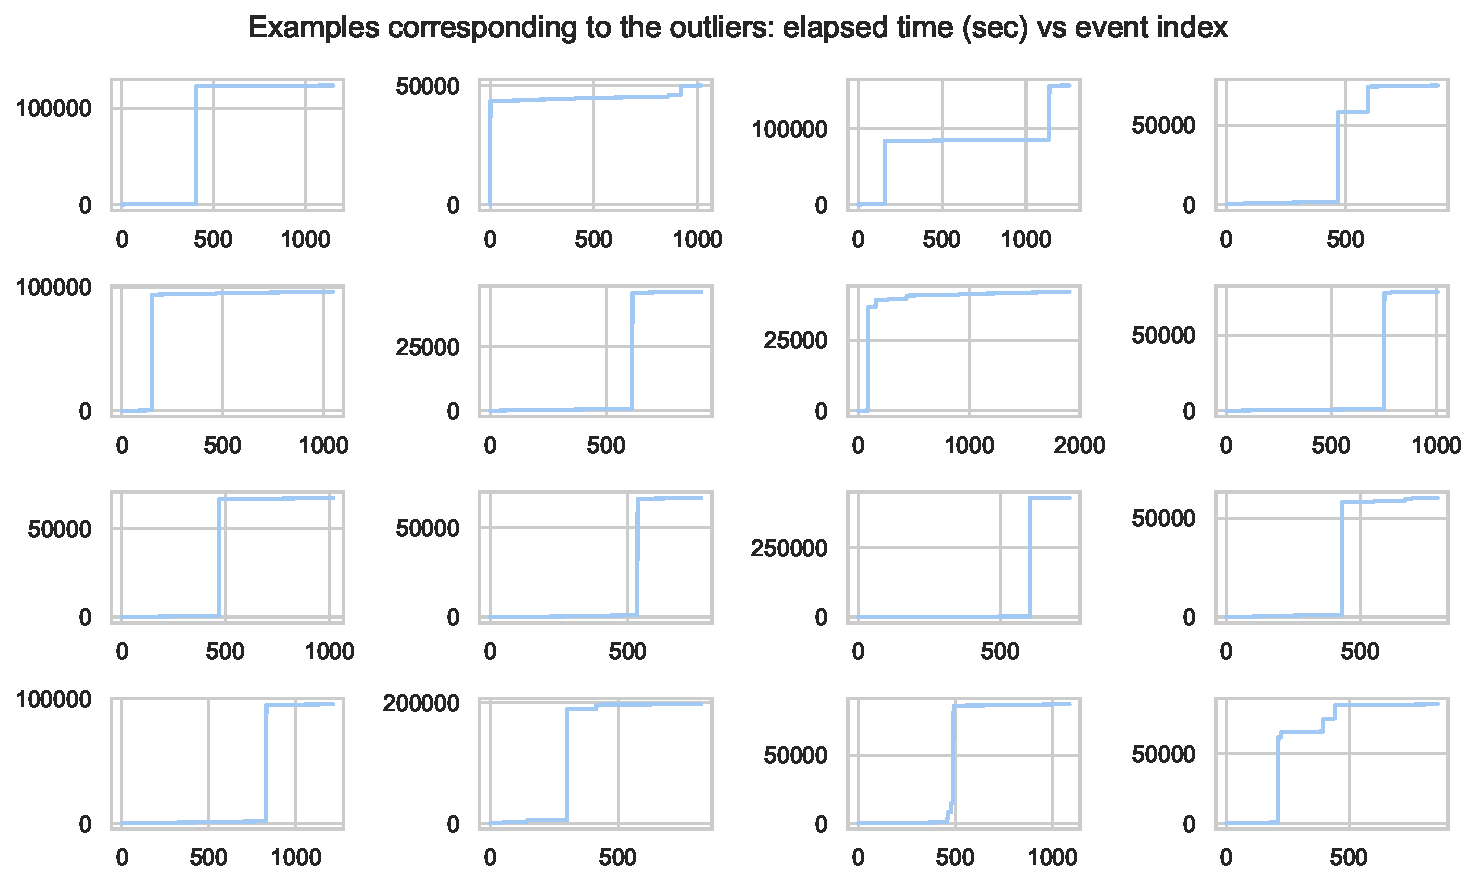
\includegraphics[width = 0.9\textwidth]{EDA_plot/elapsed_time_outliers.pdf}
        \caption{Elapsed Time of Outliers}
        \label{fig:elapsed_time_outlier}
    \end{figure}

    \subsection{Event Name and Name}
    There are 11 unique event names and 6 unique names, in the following bar charts and pivot table, we can see events are consist of 3 types, namely \textit{checkpoint}, \textit{click} and \textit{hover}.
    \begin{figure}[H]
        \centering
        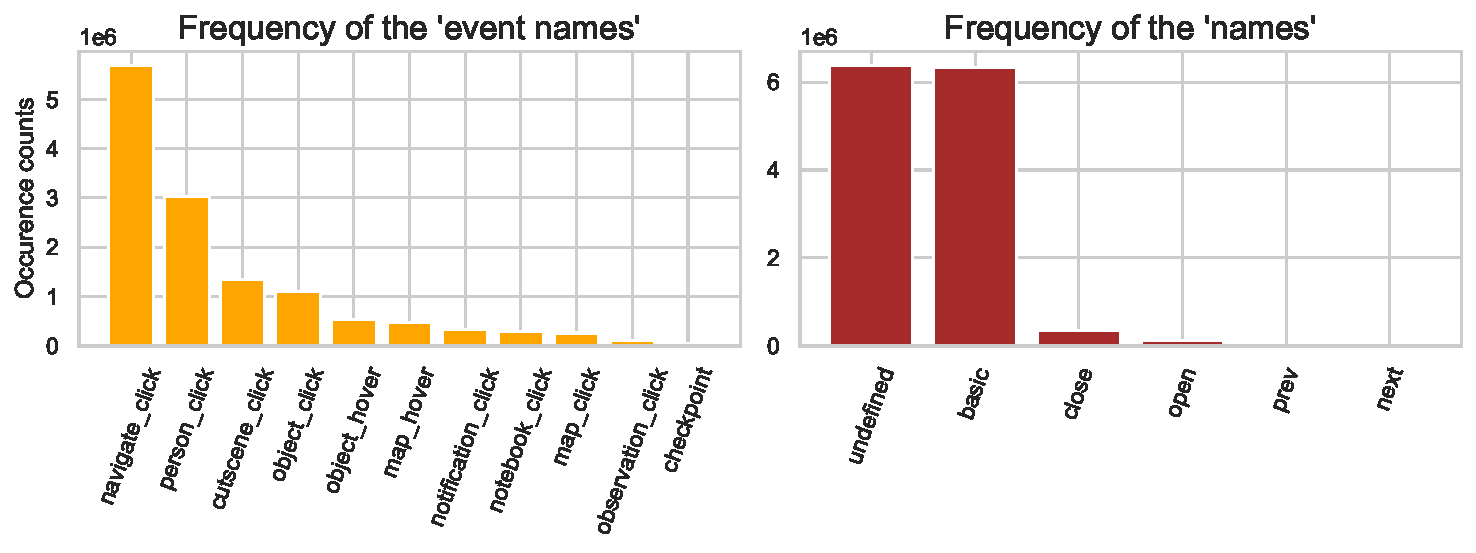
\includegraphics[width = 0.9\textwidth]{EDA_plot/event_name.pdf}
        \caption{Event Names and Names}
        \label{fig:event_name}
    \end{figure}
    \begin{figure}[H]
        \centering
        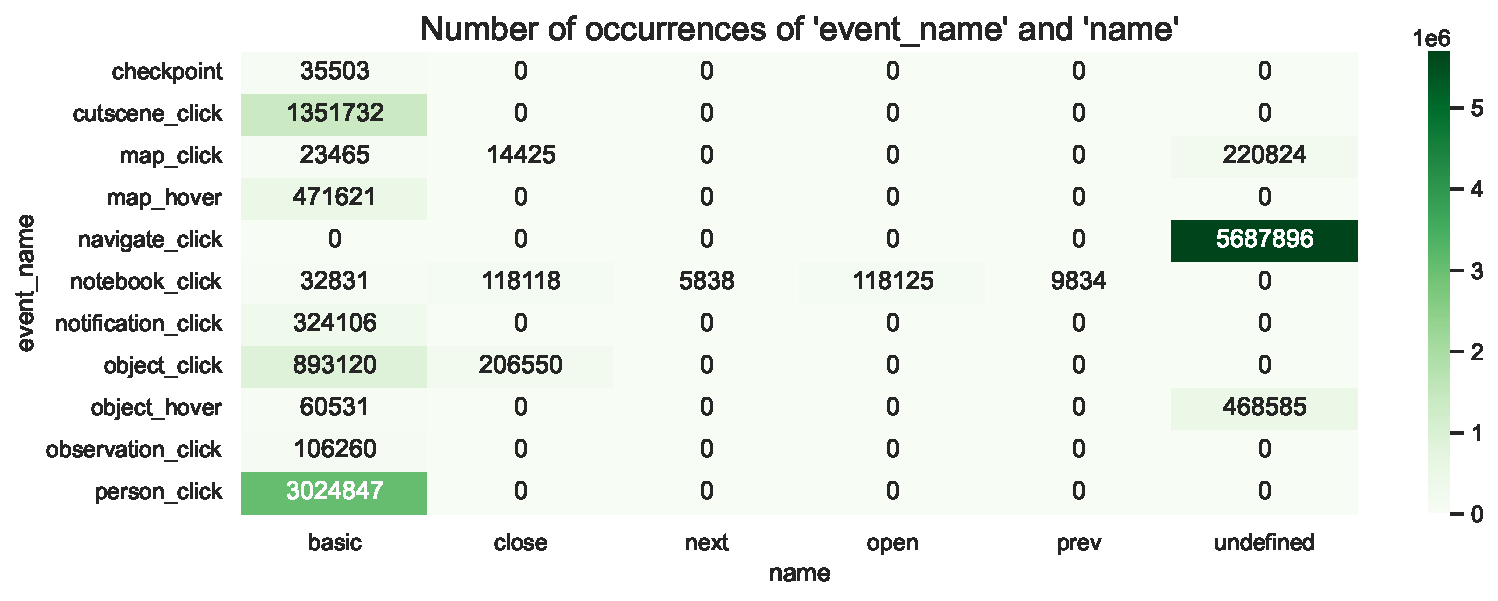
\includegraphics[width = 0.9\textwidth]{EDA_plot/event_name_pivot.pdf}
        \caption{Event Names Pivot Table}
        \label{fig:event_name_table}
    \end{figure}

    \subsection{Coordinate Features}
    \textit{room\_coor\_x}, \textit{room\_coor\_y}, \textit{screen\_coor\_x} and \textit{screen\_coor\_y} are coordinate features. We can try to plot the coordinates and have a brief understanding of what they look like. \\
    The patterns across different sessions are alike, where some noticeable clusters of clicks in certain regions. There are at least two potential button clusters, namely top left and bottom right. Players repeatedly navigated between these two clusters, resulting concentration of lines in the diagonal direction. These coordinates are probably a wealth of information, however in order to utilize it, that requires higher machine learning techniques. For example, treat it as image and use computer vision to analysis.
    \begin{figure}[H]
        \centering
        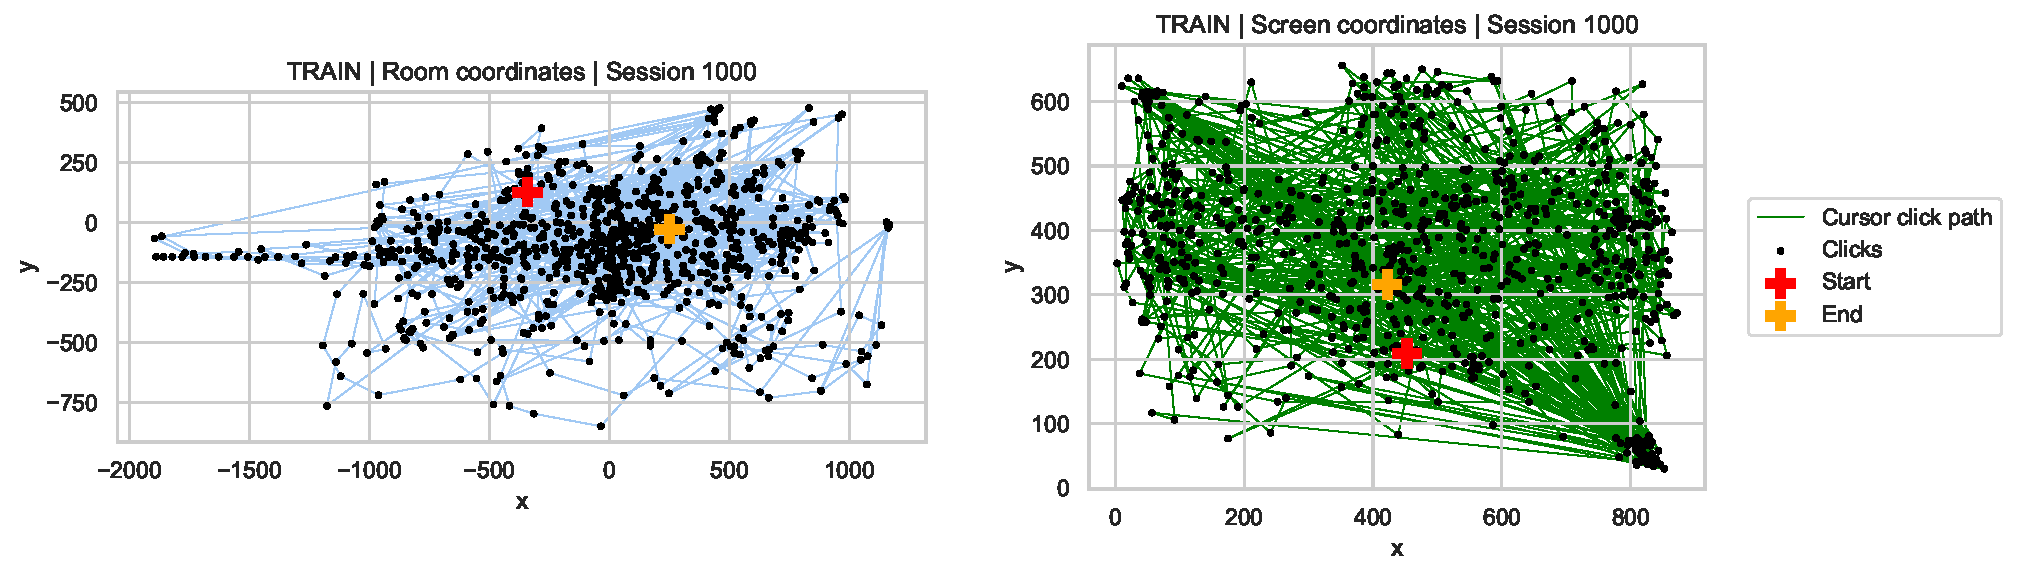
\includegraphics[width = 0.9\textwidth]{EDA_plot/corrdinates_1000.pdf}
        \caption{Coordinate Features}
        \label{fig:coordinate}
    \end{figure}

    \subsection{Labels}
    As the target of our prediction task, the goal is the predict the whether the session have correct answer on specific question. In total, about 70\% correct and 30\% incorrect, indicate that the dataset is slightly imbalanced.
    \begin{figure}[H]
        \centering
        \begin{minipage}{0.5\textwidth}
            \centering
            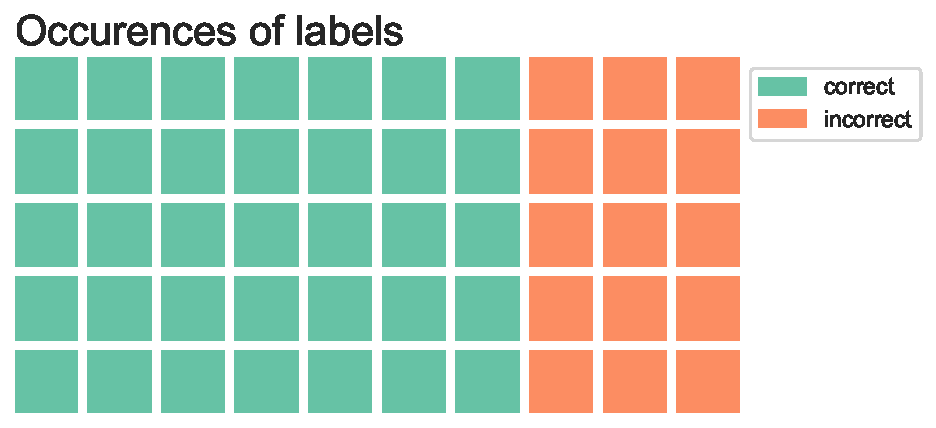
\includegraphics[width=\textwidth]{EDA_plot/labels.pdf} % first figure itself
            \caption{Occurences of Labels}
        \end{minipage}\hfill
        \begin{minipage}{0.5\textwidth}
            \centering
            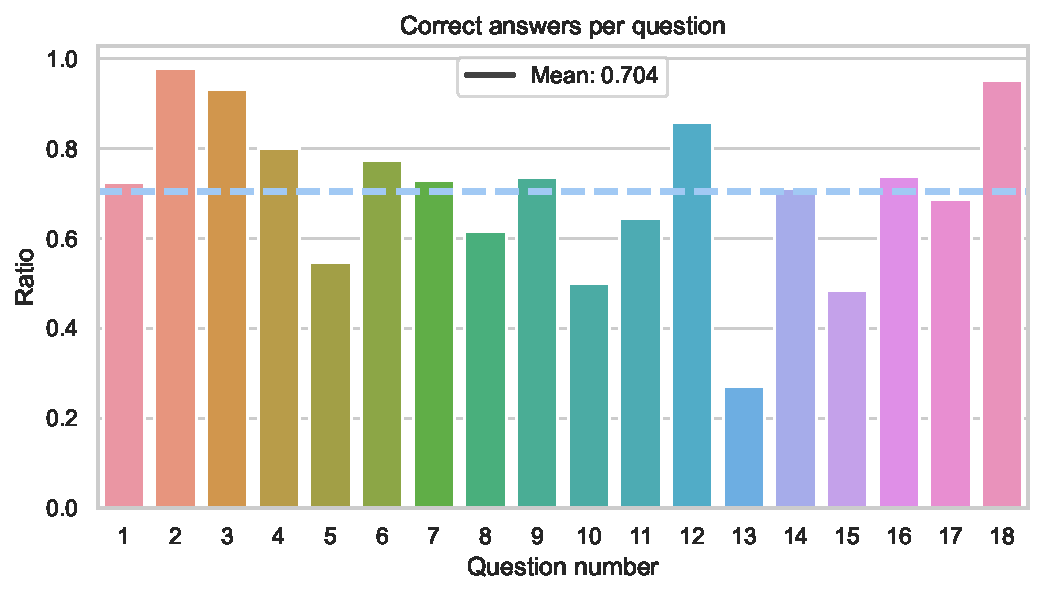
\includegraphics[width=\textwidth]{EDA_plot/correct_ratios.pdf} % second figure itself
            \caption{Correct Ratios}
        \end{minipage}
    \end{figure}
    
    \section{Data Preparation for Model Training}
    In order to use time series log data for model training, it is necessary to perform data preparation and feature engineering. This could be done by aggregating the data into a session-wise level, that is aggregating each session into one row, which can be used as input for the model. To handle this huge training dataset, Python library \href{https://www.pola.rs/}{Polars}\footnote{Polars is a lightning fast DataFrame library/in-memory query engine. Its embarrassingly parallel execution, cache efficient algorithms and expressive API makes it perfect for efficient data wrangling, data pipelines, snappy APIs and so much more.} \cite{polars} is used instead of the commonly used \textbf{Pandas}, as \textbf{Polars} performs much faster on data manipulation on large dataset. Some processes are explained in the following subsection, for the whole procedure, please refer to \texttt{XGB\_model.ipynb}.

    \subsection{Feature Engineering}
    \subsubsection{Numerical Features}
    7 numerical features are selected, ['page', 'room\_coor\_x', 'room\_coor\_y', 'screen\_coor\_x', 'screen\_coor\_y', 'hover\_duration', 'elapsed\_time\_diff']. Each numerical features are then used to compute additional statistical features such as various quantiles, minimum, maximum, mean, and standard deviation for each numerical feature. For elapsed time and coordinates, new columns are calculated base on the different from last record over ["session\_id", "level\_group"]

    \subsubsection{Categorical Features}
    5 categorical features are selected, ['event\_name', 'name', 'fqid', 'room\_fqid', 'text\_fqid']. Minimum, maximum, mean, and standard deviation are then calculated for the elapsed time difference over each categorical features. Furthermore, some further features are calculated based on specific group level.
    
    \subsection{Preprocessed Datasets}
    The feature engineering procedure is separately perform by \textit{level\_group}: ['0-4', '5-12', '13-22'] which is the level group of the question, then 3 datasets are generated. After dropping features with $> 90\%$ missing ratio and features only have single unique value, the datasets contain 599, 914 and 1059 features respectively in each level group, all contain 11,779 rows representing every unique sessions.

    \section{Machine Learning Model Approach}
    The challenge at hand can be framed as a binary classification problem, wherein the goal is to accurately classify player in each question into one of two possible categories, namely correct and incorrect. Various machine learning models can be utilized to address this task, including logistic regression, deep neural networks, and decision trees. Given the need to strike a balance between model complexity and computational efficiency, we have chosen to utilize a decision tree model in this project. This approach will enable us to effectively and efficiently classify instances based on relevant features and their associated information gain.

    \subsection{Decision Tree Model Specifications}
    
    \subsection{Group Fold Cross Validation}

    \section{Model Evaluation}

    \subsection{Optimal Prediction Threshold}

    \newpage
    \subsection{F1 Score}
    \begin{figure}[H]
        \centering
        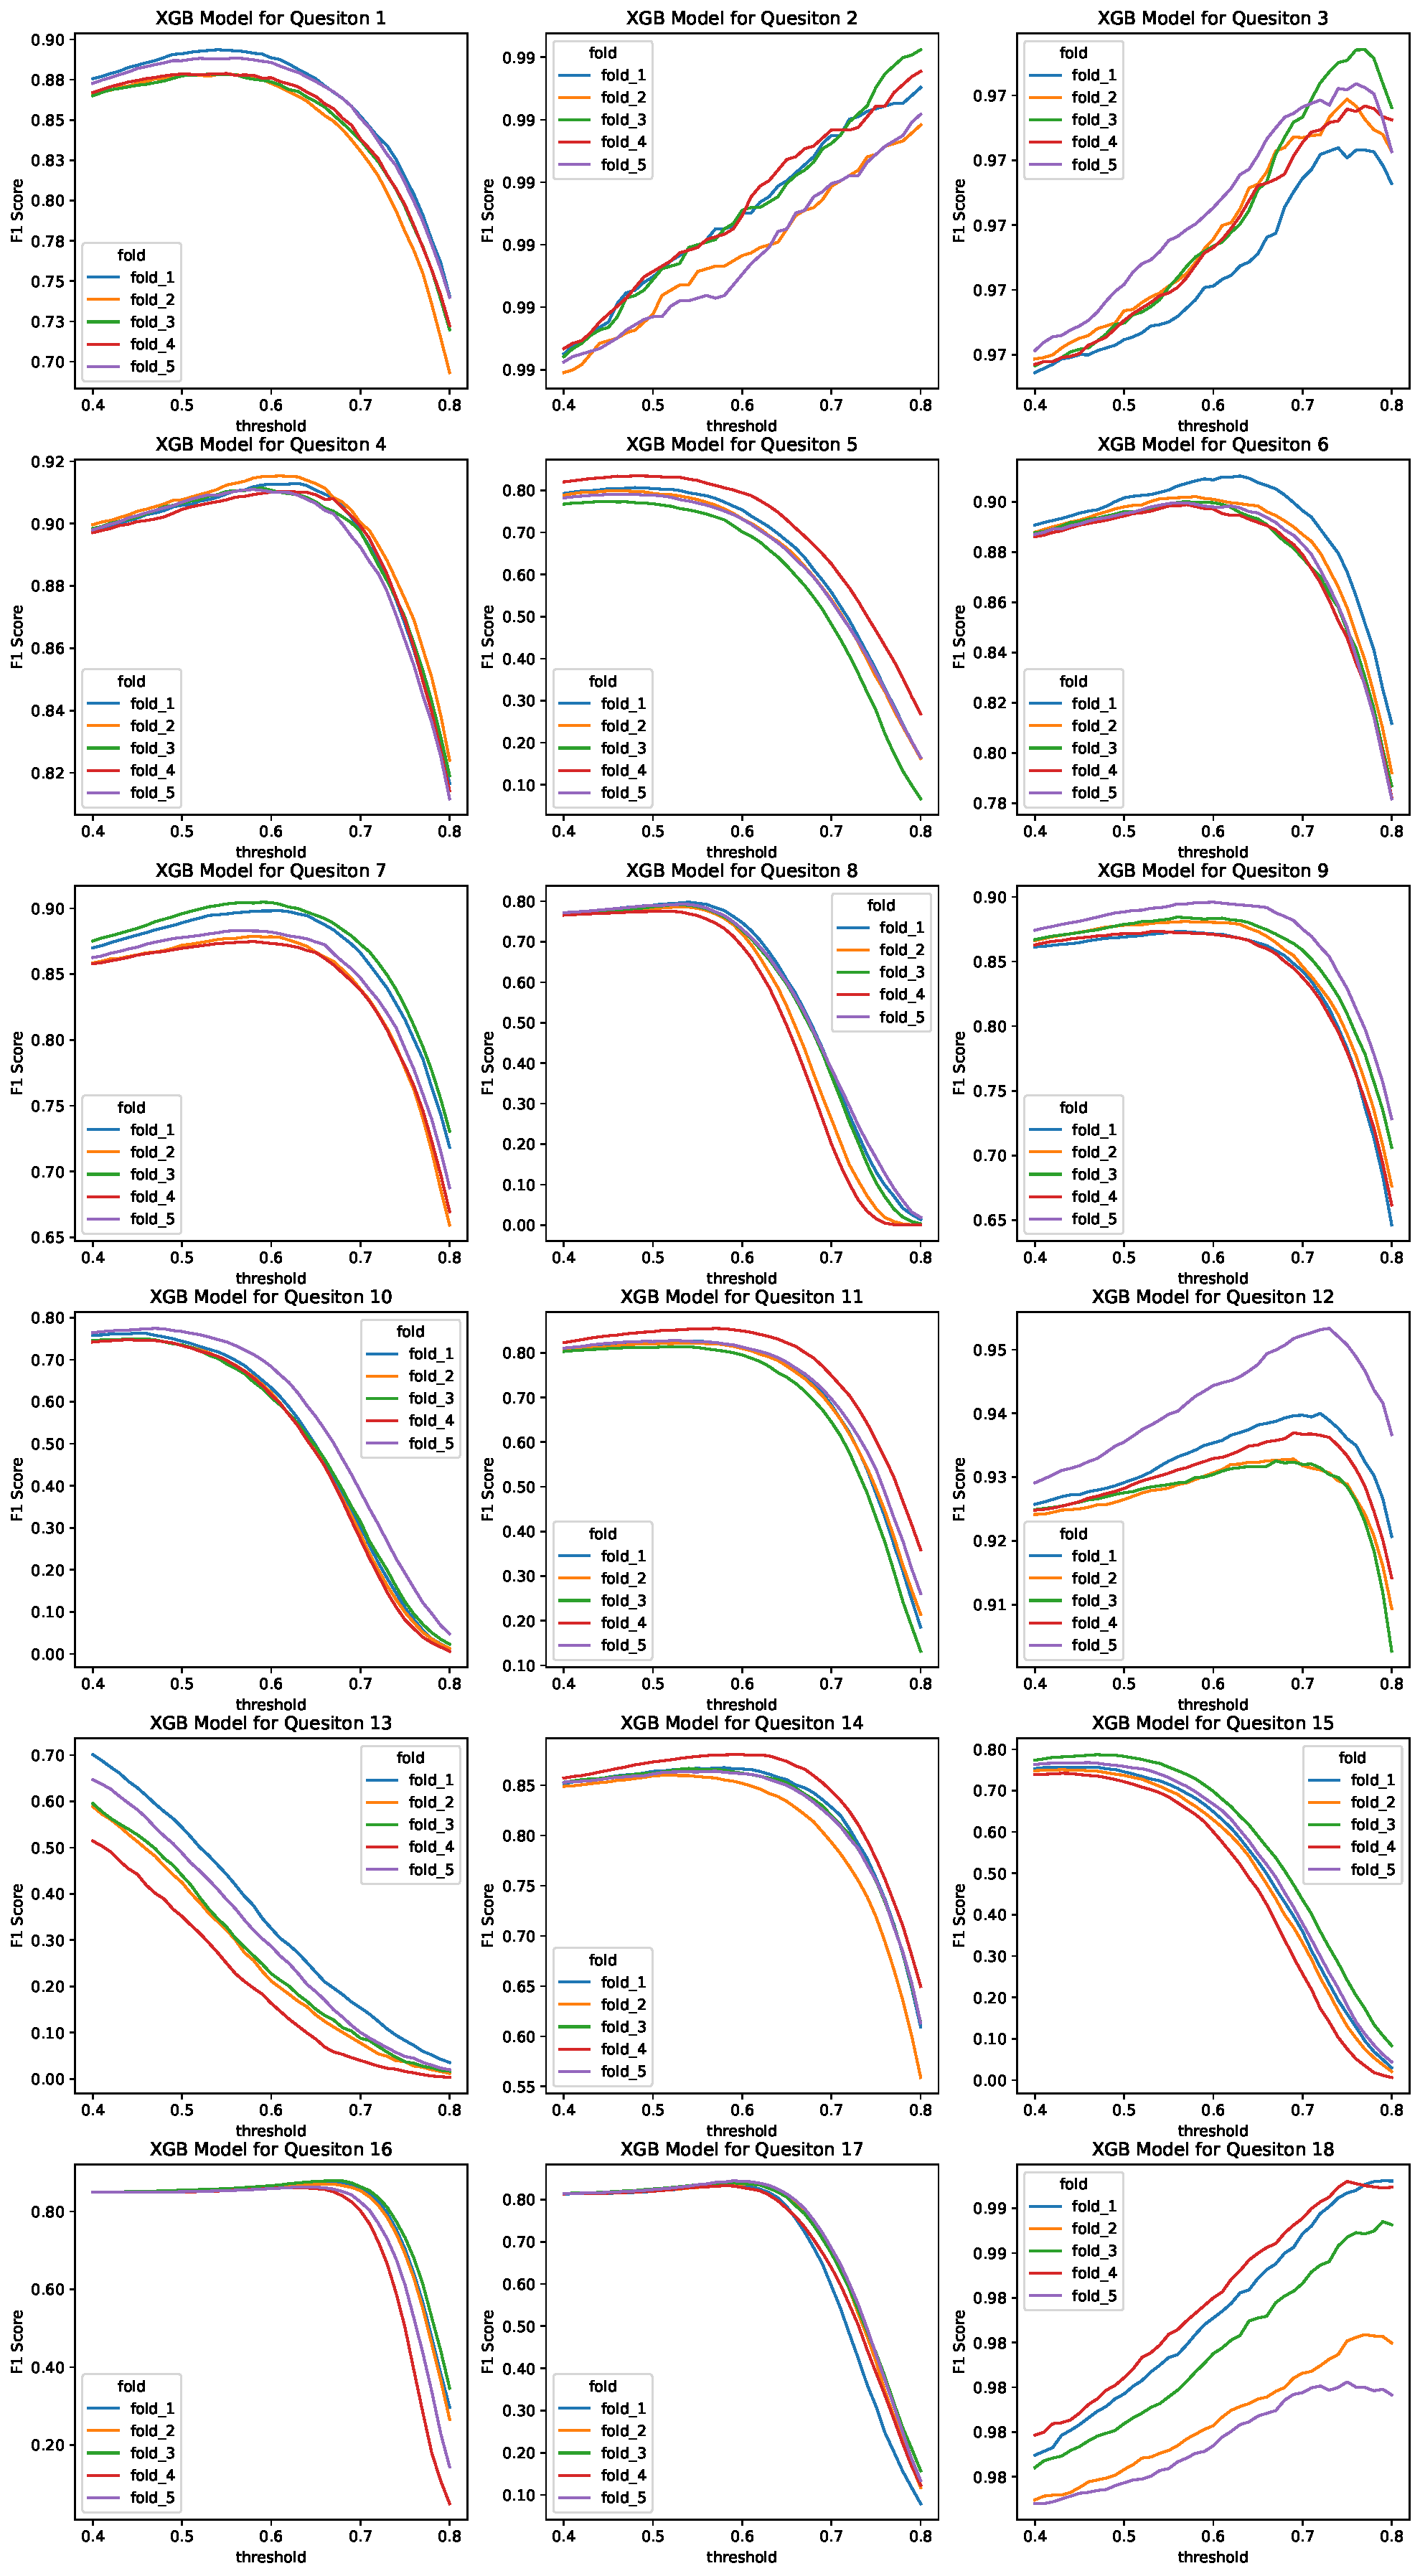
\includegraphics[width = 0.9\textwidth]{model_plot/f1_threshold.pdf}
        \caption{F1 Score vs Threshold}
        \label{fig:f1_score}
    \end{figure}

    \section{Conclusion}

    \subsection{Possible Improvement}

    \newpage
    \section{Bibliography}
    \nocite{simple_xgb, detailed_eda}
    
    \bibliographystyle{unsrt}
    % \bibliographystyle{plain} % We choose the "plain" reference style
    \bibliography{refs} % Entries are in the refs.bib file

    \newpage
    \section{Appendix}
    \subsection{Training Dataset Features}
    \label{appendix:training}
    \begin{table}[H]
        \centering
        \begin{tabular}{l|l}
            \textbf{Feature} & \textbf{Description} \\ \hline
            session\_id & the ID of the session the event took place in \\
            index & the index of the event for the session \\
            elapsed\_time & time has passed (in ms) between the start of the session and when the event was recorded \\
            event\_name & the name of the event type \\
            name & the event name (e.g. identifies whether a notebook\_click is is opening or closing the notebook) \\
            level & what level of the game the event occurred in (0 to 22) \\
            page & the page number of the event (only for notebook and related events) \\
            room\_coor\_x & the coordinates of the click in reference to the in-game room (only for click events) \\
            room\_coor\_y & the coordinates of the click in reference to the in-game room (only for click events) \\
            screen\_coor\_x & the coordinates of the click in reference to the player’s screen (only for click events) \\
            screen\_coor\_y & the coordinates of the click in reference to the player’s screen (only for click events) \\
            hover\_duration & how long (in milliseconds) the hover happened for (only for hover events) \\
            text & the text the player sees during this event \\
            fqid & the fully qualified ID of the event \\
            room\_fqid & the fully qualified ID of the room the event took place in \\
            text\_fqid & the fully qualified ID of the \\
            fullscreen & whether the player is in fullscreen mode \\
            hq & whether the game is in high-quality \\
            music & whether the game music is on or off \\
            level\_group & which group of levels - and group of questions - this row belongs to (0-4, 5-12, 13-22) \\
        \end{tabular}
        \caption{All Features of Training Dataset}
        \label{tab:training_features}
    \end{table}
    
\end{document}